\documentclass{bioinfo}
\copyrightyear{2011}
\pubyear{2011}
\raggedend
\usepackage{hyperref}
\hypersetup
{ % We don't want the hideous colored borders around the hyperlinks
  colorlinks=false,
  pdfborder={0,0,0},
}

\begin{document}
\firstpage{1}

\title[Protein fold classification]{Protein fold classification incorporating additional evolutionary information from phylogenetic profiles}
\author[Standage]{Daniel S. Standage}
\address{Department of Genetics, Development, and Cell Biology, Iowa State University, Ames, IA 50011}

\history{December 15, 2011}

\maketitle

\begin{abstract}
\noindent \textbf{Motivation}: Homology modeling has emerged as an effective method for predicting the structure of a protein from sequence data. However, these approaches perform poorly for proteins that have very low sequence similarity with any other proteins in public structure databases. Determining structural similarity without relying on sequence similarity could provide a huge benefit for the prediction of tertiary structures. \\
\noindent \textbf{Results}: I extended the previously published PFRES method for protein fold classification from low identity sequences. In addition to PSI-BLAST profile-based composition vectors and secondary-structure-based features, this new method takes advantage of evolutionary information about each protein encoded in a phylogenetic profile. My new method does not provide a significant improvement over published methods as is, but it demonstrates the potential for significant improvement given enough training data. \\
\noindent \textbf{Supplementary information}: Documentation and code describing how the feature calculations were performed and how the classifiers were trained and evaluated is available at \url{http://goo.gl/oRpdR}.
\end{abstract}

\section*{Introduction}
Recent developments in the field of genomics, particularly in the realm of genome and transcriptome sequencing, have led to an explosion of sequence data.
While DNA and protein sequences are valuable for a wide variety of analyses, elucidation of protein structure is often required for a deep understanding of gene/protein function at the biochemical and molecular level.
Current methods for protein structure determination are quite accurate, but expensive, time-consuming, complicated, and extremely low-throughput.

Homology modeling has emerged as an effective and fairly accurate method for predicting the structure of a protein for which only the primary sequence is available.
This approach uses sequence alignment scores to search a database of protein sequences with resolved 3-dimensional structures and identify a close homolog.
Once the best homolog is identified, its structure serves as a template for predicting the structure of the query protein.

The limitation of this approach is that many proteins have very little sequence similarity to any of the proteins for which structural data is available.
These sequences represent an increasingly substantial proportion of all protein sequences.
Structural prediction methods that do not depend on sequence similarity would be a very valuable resource.

Recent efforts by databases such as SCOP \citep{Andreeva} and CATH \citep{Orengo} have provided the community with comprehensive, hierarchical organization of proteins for which both sequential and structural data are available.
The SCOP database classifies each protein using the following hierarchical levels (from general to specific): \textit{class}, \textit{fold}, \textit{superfamily}, and \textit{family}.
At the fold classification level, proteins show clear structural similarity, although the sequence similarity between proteins with the same fold classification can be quite low.

Several studies \citep{Ding,Shen,Chen} have applied machine learning to classify proteins based on a variety of features related to amino acid composition, predicted secondary structure, biochemical properties, and evolutionary profiles.
The most recent work by Chen and Kurgan (2007), the PFRES method, improved on previous protein fold classification methods by combining secondary-structure-based features with a PSI-BLAST profile-based composition vector (PCV).
This PCV offers additional evolutionary information not captured in the more traditional composition vector (CV), improving the accuracy of the machine learning classifiers.

For this project, I explored an extension to the PFRES method that incorporates additional evolutionary information from phylogenetic profiles.
Previous studies \citep{Pellegrini,Wu} have demonstrated that phylogenetic profile analysis can be used to identify genes involved in similar biochemical pathways, structural complexes, etc.
These profiles capture the phylogenetic distribution of a gene in a set of reference genomes---genes with similar presence/absence patterns among these reference genomes will have very similar phylogenetic profiles.
Here I document the methods I used to reproduce the PFRES results, to extend the PFRES method by incorporating phylogenetic profiles, and to compare my results with the results previously reported by the PFRES method.

%\begin{methods}
\section*{Materials \& Methods}

\subsection*{Training and testing data}
Training data consists of 313 protein domains, representing 27 fold classifications within the SCOP ontology \citep{Andreeva} (the 27 most populated folds).
To accurately predict the behavior of the machine learning classifiers on protein sequences with low sequence similarity to resolved proteins, this data set was constructed such that the similarity between any pair of sequences is $<35\%$.

Model evaluation was performed on two test sets.
Test set 1 includes 385 protein domains from the same 27 folds as the training set, and was constructed such that no sequence in test set 1 shared $>35\%$ similarity with any sequence in the training set.
Test set 2 includes 908 domains, also from the same 27 folds, and constructed such that no sequence from test set 2 shared $>35\%$ similarity with any sequence from the other two sets.

The training set and test set 1 were designed by Ding and Dubchak as described in \citep{Ding,Shen}, and can be downloaded from \url{http://www.csbio.sjtu.edu.cn/bioinf/PFP-FunDSeqE/Data.htm}.
Test set 2 was designed by Shen and Kurgan as described in \citep{Chen}, and can be downloaded from \url{http://biomine.ece.ualberta.ca/PFRES/PFRES.htm}.

\subsection*{Feature Calculation}

\subsubsection*{PSI-BLAST profile-based composition vector}
The first protein fold classification methods used a composition vector (CV) to capture the amino acid composition of a given protein sequence.
This composition vector is defined as
\[ \left(\frac{n_1}{L}, \frac{n_2}{L},...,\frac{n_{20}}{L} \right) \]
where $L$ is the length of the sequence and $n_i$ corresponds to the number of times the $i^{th}$ amino acid appears in the sequence.

The PFRES method \citep{Chen} describes an alternative to the CV that captures not only amino acid composition but also evolutionary information from a PSI-BLAST profile.
The PSI-BLAST algorithm aligns the query protein to a database of reference sequences.
It subsequently aligns the query protein to the sequence hits and builds a position-specific substitution matrix (PSSM) from the resulting multiple sequence alignment.
The PSI-BLAST profile (PSSM) is an $L \times 20$ matrix containing not only the composition of the query protein but also the composition of evolutionarily related sequences.

My method utilizes the PSI-BLAST profile-based composition vector (PCV) as defined in the PFRES method.
Given the PSSM $a_{ki}$ for a protein, the PCV is defined as
\[ PCV_i = \sum_{k=1}^{L}\frac{\max{(a_{ki},0})}{L} \hspace{12px} (i=1,2,...,20) \]
where $L$ is the length of the protein.
The supplementary materials include the parameters with which PSI-BLAST was run and the software used to convert the resulting PSSM into a PCV.

\subsubsection*{Secondary-structure-based features}
Fold classification methods also typically take advantage of protein secondary structure.
The PFRES method defines several features computed from secondary structure predictions that I likewise implemented in my feature representation.
The PSI-PRED program \citep{Jones} was used to generate secondary structure predictions, and the supplementary materials include details on how the software was run and how the following features were computed; also, see Figure \ref{SSGraphic}.

Secondary structure content (SSC) refers, unsurprisingly, to the content of the 3 predicted secondary structure classes (helix = $H$, strand = $E$, coil = $C$) in the protein.
Formally, SSC is defined as
\[ SSC_m = \frac{COUNT_m}{L} \]
where $m \in \{H, E, C\}$, $COUNT_m$ refers to the number of predictions of class $m$ in the protein, and $L$ refers to the protein length.

A distinct secondary structure segment (DSSS) refers to a contiguous set of amino acids which have been classified with the same secondary structure designation.
My method uses the number of distinct helix, strand, and coil structures present in the protein, as well as counts for all possible arrangements of 3 adjacent DSSSs.
Because extremely short DSSSs have a greater possibility of being incorrectly classified, filters were used to exclude any DSSSs that fell below a given threshold ($H=7$, $E=5$, $C=6$).
The method used to determine these thresholds was described in the PFRES method \citep{Chen}.

\begin{figure} \centering
  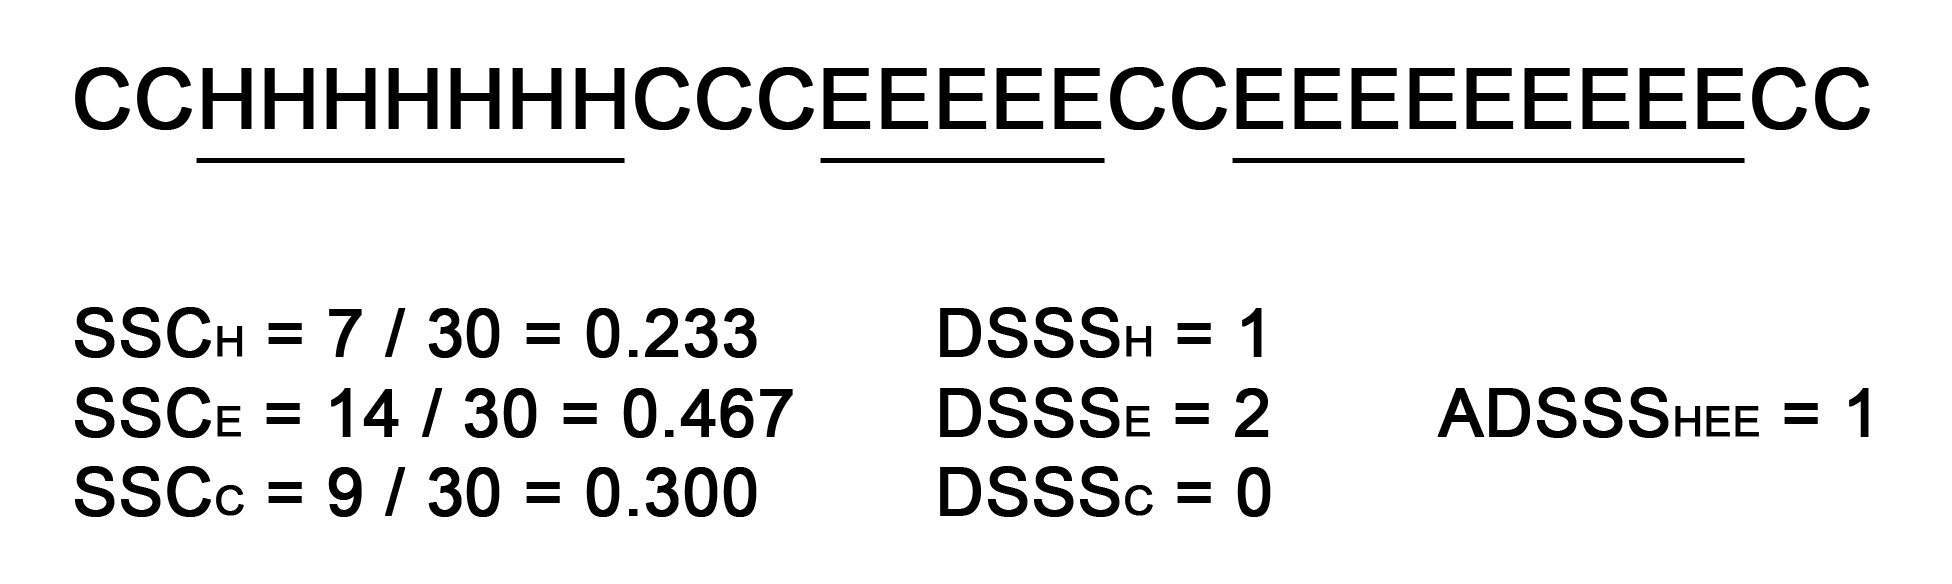
\includegraphics[width=240px]{../ss.png}
  \caption{Secondary structure predictions for a short, hypothetical protein domain are shown above to demonstrate how secondary-structure-based features are calculated. The SSC features capture the composition of the 3 structural classes, the DSSS features capture the number of distinct structural segments, and the ADSSS feature captures the number of adjacent DSSS 3-mers. Note that although 9 amino acids have a $C$ structural designation, $DSSS_C$ is still 0 since no contiguous segments of $C$ are long enough. Note also that there are a total of 27 ADSSS features (every possible arrangement of $H$, $E$, and $C$), but only one is present in this example. The ADSSS features not shown have a value of 0.}
  \label{SSGraphic}
\end{figure}

\subsubsection*{Phylogenetic profiles}
The primary focus of my project was to determine whether phylogenetic profile information can be used to improve protein fold classification.
Phylogenetic profiles were first described as a method for predicting gene function \citep{Pellegrini} and are based on the assumption that genes related by function (for example, in the same biochemical pathway or structural complex) will be inherited and lost together through the course of evolutionary time.
Phylogenetic profiles are designed to represent this idea mathematically, and have been successfully used with a variety of scoring and clustering techniques to infer gene/protein function \citep{Kensche}.

Given a set of $n$ reference genomes $G = \{G_1, G_2, ..., G_n\}$, the phylogenetic profile of a gene $g$ (or rather of its protein product) is a binary string $p = p_1 p_2 ... p_n$ such that $p_i = 1$ if genome $G_i$ includes a homolog of $g$ and $p_i = 0$ otherwise.

In the past, I have typically used a very large set of reference genomes when building phylogenetic profiles ($n$ on the order of 1000).
However, given the size of the training data set for this protein fold classification problem, I had to use a much more conservative $n$ so as to maintain a high ratio of data instances to features.
I therefore (somewhat subjectively) selected $n=12$ as the number of references organisms to use when building phylogenetic profiles.

Given this small $n$, and unsure as to whether these 12 genomes should be distributed broadly or narrowly across the phylogenetic spectrum, I generated two alternative protein databases from which phylogenetic profiles can be built.
The first includes proteins from 12 organisms that represent the most possible diversity in eukaryotic lineages.
The second includes proteins from 12 organisms within the dicotyledons, a group of flowering plants which have a much closer evolutionary relationship (see Table \ref{PhyloProfTable}).
Using these two databases and the \texttt{blastp} program, I generated two phylogenetic profiles for each protein in the training set and the two test sets.
Subsequent fold classification tasks were performed twice (each time using only one of these two phylogenetic profiles) so as to enable comparison of the relative performance benefit of the two profiles.

The procedure for constructing the two reference data sets, as well as the code used to generate the phylogenetic profiles, can be found in the supplementary materials.

\begin{table} \centering
  \begin{tabular}{ l l }
    \hline
    \multicolumn{1}{c}{\textbf{Eukaryotes}} & \multicolumn{1}{c}{\textbf{Dicots}} \\ \hline
    %\textbf{Species} & \textbf{Abbrev.} & \textbf{Common Name} \\ \hline
    \textit{Arabidopsis thaliana} & \textit{Arabidopsis thaliana} \\
    \textit{Aspergillus nidulans} & \textit{Carica papaya} \\
    \textit{Cryptosporidium parvum} & \textit{Cucumis sativus} \\
    \textit{Danio rerio} & \textit{Glycine max} \\
    \textit{Drosophila melanogaster} \hspace{15px} & \textit{Lotus japonicus} \\
    \textit{Eremothecium gossypii} & \textit{Manihot esculenta} \\
    \textit{Homo sapiens} & \textit{Medicago trunculata} \\
    \textit{Mus musculus} & \textit{Mimulus guttatus} \\
    \textit{Physcomitrella patens} & \textit{Populus trichocarpa} \\
    \textit{Plasmodium falciparum} & \textit{Prunus persica} \\
    \textit{Saccharomyces cerevisiae} & \textit{Ricinus communis} \\
    \textit{Zea mays} & \textit{Solanum lycoparsicum} \\ \hline
    %\multicolumn{3}{c}{}
  \end{tabular}
  \vspace{5px}
  \caption{Phylogenetic profiles represent the phylogenetic distribution of a gene in a set of reference organisms. Not knowing whether profiles with more or less phylogenetic diversity would provide better discrimination for fold classification, I generated two databases from which phylogenetic profiles could be built. The first contains proteins from a wide range of eukaryotic species, while the second contains proteins only from within the dicot clade. I then generated two phylogenetic profiles for each protein in the training and test data (one profile from each database). Subsequent feature selection and classification tasks were performed twice so as to evaluate the relative performance benefit of these phylogenetic profiles.}
  \label{PhyloProfTable}
\end{table}


\subsection*{Feature Selection}
For the purposes of classification, each protein is represented by a 66-dimensional vector comprising the PCV (20 features), secondary-structure-based features (33 features), the protein length (1 feature), and the phylogenetic profile (12 features); see Table \ref{FeatureSpaceTable}.
Given the limited size of the training and test data sets, feature selection was used to reduce the dimensionality of the data to maintain a high ratio of data instances to features.

The Weka machine learning workbench was used to perform feature selection \citep{Eibe}. I applied the \textit{InfoGainAttribute-Eval} module with 10-fold cross-validation to the training data to sort the 66 features according to information gain.
From the entire set of features, 43 features with the best information gain values were selected; see Table \ref{FeatureSpaceTable}.

\begin{table} \centering
  \begin{tabular}{ l l l }
    \hline
    \multicolumn{1}{c}{\textbf{Characteristic}} & \textbf{\# Features} & \multicolumn{1}{c}{\textbf{Selected Features}} \\ \hline
    PCV    & 20 & 20 \\
    SSC    & 3  & 3 \\
    DSSS   & 3  & 3 \\
    ADSSS  & 27 & 10 \\
    Length & 1 & 1 \\
    Phylogenetic profile & 12 & 6 \\
    \textbf{Total} & \textbf{66} & \textbf{43} \\ \hline
  \end{tabular}
  \vspace{5px}
  \caption{Summary of the feature space used for protein fold classification. For each protein in the training and test sets, the following characteristics were calculated: PSI-BLAST profile-based composition vector (PCV), secondary structure content (SSC), number of distinct secondary structure segments (DSSS), DSSS 3-mers (ADSSS), length, and phylogenetic profile. Two feature spaces were calculated for each protein (to incorporate two different phylogenetic profiles). The feature spaces were reduced to 43 dimensions using an information-gain-based feature selection module. The resulting feature spaces were identical except for the 6 phylogenetic-profile-based features.}
  \label{FeatureSpaceTable}
\end{table}

\subsection*{Training and evaluation of machine learning classifiers}
The PFRES method reported results for a variety of machine learning classifiers, as well as ensemble classifiers that combine predictions from individual algorithms.
I used the best-performing classifiers described by this study to enable comparison of my results against a reference.
Given the amount of time that has passed since the PFRES method was published, I also reproduced their experiment so as to accurately account for updates that have been made to databases and software in the last few years.
The results of my new tests were compared both against the original published PFRES results as well as the results of my PFRES reproduction.

The individual classification algorithms considered were Random Forest (250 trees), Support Vector Machine (RBF kernel, $\gamma = 0.8$, $C = 5.0$), and Kstar (global blend = 96).
Additionally, I tested a voting-based ensemble classifier that combines predictions from the previous 3 classifiers using a majority vote of the corresponding classification predictions.

Implementations of all aforementioned classifiers are available in the Weka machine learning workbench \citep{Eibe}, and Weka was used for all training and evaluation tasks.
Each of the classifiers were trained using the training data and then evaluated using both test data sets.

%\end{methods}


\section*{Results}
Four machine learning classifiers were trained using the training data set (following feature selection).
After the classifiers were trained, both test sets were evaluated on the trained models.
A summary of the results of these tests are shown in Table \ref{ResultsTable}.

For both Test 1 and Test 2, each classifier trained with eukaryotic phylogenetic profiles outperformed the corresponding classifier trained with dicot phylogenetic profiles.
For Test 1, the Random Forest algorithm had the best performance of the individual classifiers with an accuracy of 65.8\%.
This provides a very slight improvement over the results of the reproduced PFRES method, whose performance is approximately 1\% below the published results.
The Kstar classifier had an accuracy of 63.2\%, which is the precise performance of the reproduced PFRES method, although a few percent below the published results.
On the other hand, the SVM classifier had an accuracy of 61.4\%, which is several percent below both the reproduced PFRES method and the published PFRES results (66.8\% and 66.1\%, respectively).
The ensemble classifier achieved an accuracy of 65.8\% (same as Random Forest), compared to 67.1\% in the reproduced PFRES method and 68.4\% in the published PFRES results.

For Test 2, the Random Forest algorithm had the best performance of all classifiers with an accuracy of 64.6\%, an improvement over both the reproduced and published PFRES results.
The Kstar classifier had an accuracy of 59.4\%, which outperforms the reproduced PFRES results but falls short of the published PFRES performance.
The SVM classifier had a significant performance drop in comparison to both the reproduced and published PFRES results: 53.1\% versus 62.9\% and 62.4\%, respectively.
The ensemble classifier achieved an accuracy of 62.7\%, barely edging out the results of the reproduced PFRES method.

\begin{table} \centering
  \begin{tabular}{ c c c c c }
    \hline
    \textbf{Classifier} & \textbf{Eukaryotes} & \textbf{Dicots} & \textbf{PFRES} & \textbf{Published} \\ \hline
    \multicolumn{1}{l}{RF} & \multicolumn{4}{c}{\hspace{15px}} \\
    \multicolumn{1}{r}{Test 1} & \textbf{65.8\%} & 62.9\% & 65.5\% & 66.8\% \\
    \multicolumn{1}{r}{Test 2} & \textbf{64.6\%} & 59.8\% & 64.0\% & 63.3\% \\
    \multicolumn{1}{l}{SVM} & \multicolumn{4}{c}{\hspace{15px}} \\
    \multicolumn{1}{r}{Test 1} & 61.4\% & 54.8\% & 66.8\% & 66.1\% \\
    \multicolumn{1}{r}{Test 2} & 53.1\% & 51.1\% & 62.9\% & 62.4\% \\
    \multicolumn{1}{l}{Kstar} & \multicolumn{4}{c}{\hspace{15px}} \\
    \multicolumn{1}{r}{Test 1} & \textbf{63.2\%} & 57.2\% & 63.2\% & 65.0\% \\
    \multicolumn{1}{r}{Test 2} & \textbf{59.4\%} & 52.5\% & 56.7\% & 62.7\% \\
    \multicolumn{1}{l}{Ensemble \hspace{25px} ~} & \multicolumn{4}{c}{\hspace{15px}} \\
    \multicolumn{1}{r}{Test 1} & 65.8\% & 60.1\% & 67.1\% & 68.4\% \\
    \multicolumn{1}{r}{Test 2} & \textbf{62.7\%} & 56.5\% & 62.6\% & 66.4\% \\ \hline
  \end{tabular}
  \vspace{5px}
  \caption{Summary of two sets of classifier test evaluations. In both tests, a variety of classifiers trained using the training data set. Then in Test 1 and Test 2, each classifier was evaluated on Test set 1 and Test set 2, respectively. There are two copies of each data set---one with a eukaryotic phylogenetic profile, and one with a dicot phylogenetic profile. Each test was repeated so as to compare the relative performance benefit of these two phylogenetic profiles. The accuracy of the 4 classifiers tested are shown above: Random Forest (RM), Support Vector Machine (SVM), Kstar, and an ensemble classifier that combines predictions from the preceding 3 classifiers using a majority vote of the corresponding classification predictions. The \textbf{PFRES} column shows the results of my reproduction of the PFRES method, while the \textbf{Published} column shows the results of PFRES method as published in the original paper. The bold performance scores indicate where one of the new classifiers matched or outperformed the corresponding classifier from the reproduced PFRES experiment.}
  \label{ResultsTable}
\end{table}


\section*{Discussion}
\subsection*{Relative performance benefit of phylogenetic profiles}
For both tests, each classifier performed significantly better when using phylogenetic profiles derived from the eukaryotic database rather than the dicot database.
These differences were consistently in the 5-7\% range.
From this I can conclude that phylogenetic profiles representing a broad phylogenetic distribution provide more discriminatory information for protein fold classification than profiles representing a very narrow distribution.

\subsection*{Relative performance of new method to PFRES method}
Considering all classifiers across all tests, my new method matches or outperforms the previously published PFRES method in approximately half of the cases.
However, the improvements of my method are quite small and functionally insignificant.
It is important to note that my method uses a 43-dimensional feature space, while PFRES uses only 36 dimensions, so despite the fact that the PFRES method has a higher ratio of data instances to features, my method has comparable performance.

\subsection*{Future work}
In my previous work, I have typically used phylogenetic profiles derived from databases containing proteins from hundreds or thousands of organisms.
I would like to have done so for this project as well, but was severely limited by the amount of training data available.
However, the PFRES study is over 5 years old by now, and many protein structures have been deposited into public databases since then.
In the future, it would be interesting to build a training and test data set large enough to enable the incorporation of much larger phylogenetic profiles.
I expect that the performance of these classifiers would increase substantially if there were enough training data to include phylogenetic profiles that have information for 50-100 species.

\section*{Acknowledgements}
I would like to thank Dr. Robert Jernigan for steering me toward this topic. I would also like to thank Drs. Hongbin Shen and Lukasz Kurgan for helping locate and use the training and testing data for this study, and Dr. Kurgan in particular for helping me reproduce his experiments.

\begin{thebibliography}{}
\begin{raggedright}
\bibitem[Andreeva \textit{et~al}, 2004]{Andreeva} Andreeva A., Howorth D., Brenner S.E., Hubbard T.J.P., Chothia C., Murzin A.G. (2004). SCOP database in 2004: refinements integrate structure and sequence family data. \textit{Nucl. Acid Res.} 32:D226-D229.

\bibitem[Chen and Kurgan, 2007]{Chen} Chen, K. and Kurgan, L. (2007) PFRES: protein fold classification by using evolutionary information and predicted secondary structure. \textit{Bioinformatics}. \textbf{23}(21): 2843-2850.

\bibitem[Ding and Dubchak, 2001]{Ding} Ding,C.H. and Dubchak,I. (2001) Multi-class protein fold recognition using support vector machines and neural networks. \textit{Bioinformatics}, \textbf{17}, 349-358.

\bibitem[Eibe \textit{et~al}, 2004]{Eibe} Eibe F., Hall M., Trigg L., Holmes G., and Witten I. (2004) Data mining in bioinformatics using Weka. \textit{Bioinformatics}. \textbf{20}(15): 2479-2481.

\bibitem[Jones, 1999]{Jones} Jones DT. (1999) Protein secondary structure prediction based on position-specific scoring matrices. \textit{J. Mol. Biol}. \textbf{292}: 195-202.

\bibitem[Kensche \textit{et~al}, 2008]{Kensche} Kensche P.R., van Noort V., Dutilh B.E., and Huynen M.A. (2008) Practical and theoretical advances in predicting the function of a protein by its phylogenetic distribution. \textit{J. R. Soc. Interface}, \textbf{5}:151-170.

\bibitem[Orengo \textit{et~al}, 2002]{Orengo} Orengo, C. A., Bray, J. E., Buchan, D. W. A., Harrison, A., Lee, D., Pearl, F. M. G., Sillitoe, I., Todd, A. E. and Thornton, J. M. (2002), The CATH protein family database: A resource for structural and functional annotation of genomes. \textit{PROTEOMICS}, \textbf{2}: 11-21.

\bibitem[Pellegrini \textit{et~al}, 1999]{Pellegrini} Pellegrini M., Marcotte E.M., Thompson M.J., Eisenberg D., and Yeates T.O (1999) Assigning protein functions by comparative genome analysis: Protein phylogenetic profiles. \textit{PNAS}. \textbf{96}(8), 4285-4288.

\bibitem[Shen and Chou, 2006]{Shen} Shen,H.B. and Chou,K.C. (2006) Ensemble classifier for protein fold pattern recognition. \textit{Bioinformatics}, \textbf{22}, 1717-1722.

\bibitem[Wu \textit{et~al}, 2005]{Wu} Wu H., Su Z., Mao F., Olman V., and Xu Y. (2005) Prediction of functional modules based on comparative genome analysis and Gene Ontology application. \textit{Nucl. Acids Res}. \textbf{33}(9): 2822-2837.

\end{raggedright}
\end{thebibliography}

\end{document}
